\section[Introduction]{Introduction}

\begin{frame}{Why Quantum?}
Imagine you want to seat 10 fussy people at a dinner party, where there is only one optimal seating plan out of all the different possible combinations. How many different combinations would you have to explore to find the optimal?

Can you guess how many \alert{combinations}?
\end{frame}

\begin{frame}{Why Quantum?}


			
			
		
			
			\metroset{block=fill}
			
			\begin{exampleblock}{For 2 people}
				2 Total combination.
			\end{exampleblock}
			
			\begin{block}{For 5 people}
				120 Total combination.
			\end{block}
			
			\begin{alertblock}{For 10 people}
				Over 3 Million of total combination!!!
			\end{alertblock}
			
		
				
				
			
			
			
\begin{itemize}
			\item Supercomputers don't have the working \alert{memory} to hold the myriad combinations of real world problems.
			\item Supercomputers have to analyze each combination one after another, which can take a long \alert{time}.
		\end{itemize}
		
				
				

\end{frame}

\begin{frame}[fragile]{Quantum Computers}
%Until now, we’ve relied on supercomputers to solve most problems. %These are very large classical computers, often with thousands of %classical CPU and GPU cores. However, supercomputers aren’t very %good at solving certain types of problems, which seem easy at first %glance. This is why we need quantum computers.
\begin{figure}[H]
  \centering
    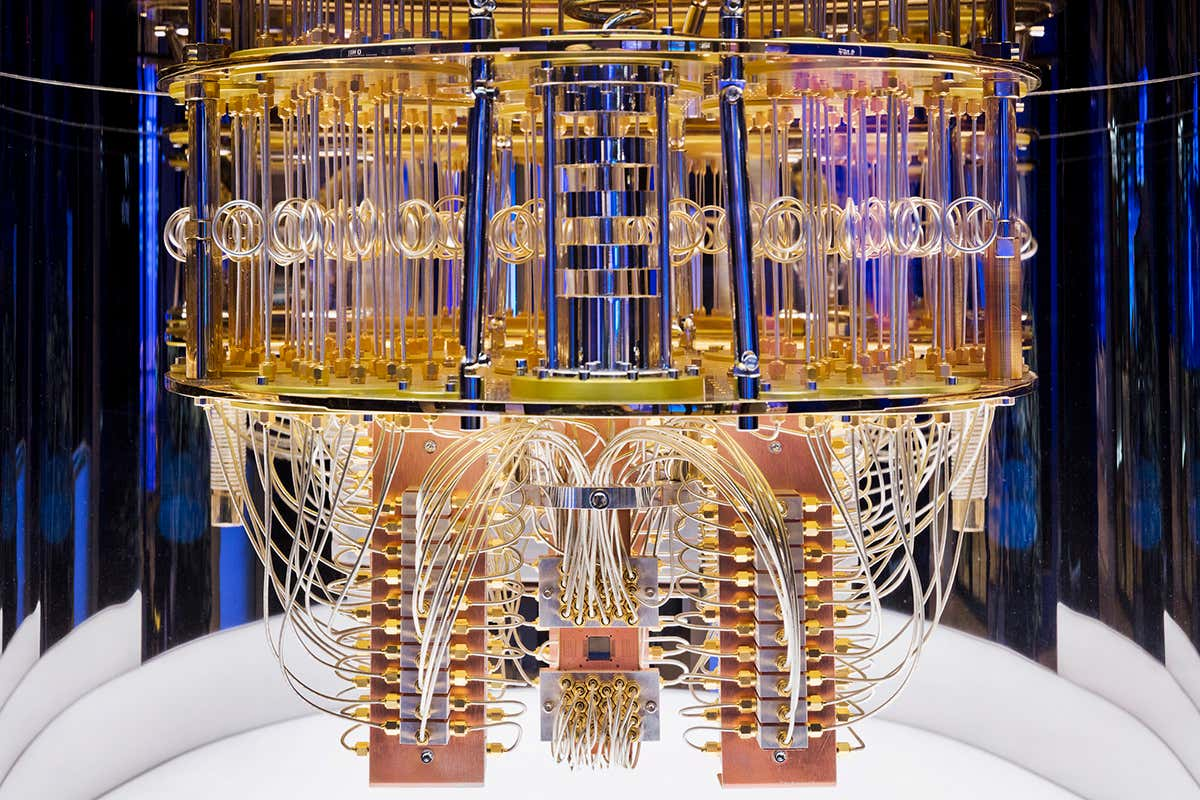
\includegraphics[width=.8\linewidth]{assets/quantum-computers-1.jpg}
    \caption{Quantum Computer}
\end{figure}

\end{frame}

\begin{frame}[fragile]{Metropolis}
	
	The \themename theme is a Beamer theme with minimal visual noise
	inspired by the \href{https://github.com/hsrmbeamertheme/hsrmbeamertheme}{\textsc{hsrm} Beamer
		Theme} by Benjamin Weiss.
	
	Enable the theme by loading
	
	\begin{verbatim}    \documentclass{beamer}
		\usetheme{metropolis}\end{verbatim}
	
	Note, that you have to have Mozilla's \emph{Fira Sans} font and XeTeX
	installed to enjoy this wonderful typography.
\end{frame}

\begin{frame}[fragile]{Sections}
	Sections group slides of the same topic
	
	\begin{verbatim}    \section{Elements}\end{verbatim}
	
	for which \themename provides a nice progress indicator \ldots
	
\end{frame}